\begin{section}{Mise en place d'un bootstrapping}
\begin{subsection}{Un point sur la sécurité}
JE N'AI PAS RETROUVÉ LE TERME UTILISÉ PAR MR. CASTAGNOS SUR LA SÉCURITÉ ICI.
CIRCULAIRE ? CYCLIQUE ? UN TRUC DE CE GENRE.\\
Nous avons vu que le système cryptographique que nous étudions est IND-CPA, ce qui est le niveau de sécurité théorique que l'on veut généralement. La première question qui se pose pour le bootstrapping est de savoir si l'on garde ce niveau de sécurité.\\
Le problème est que pour effectuer un déchiffrement homomorphe, il faut au moins un chiffré de la première clé secrète par la deuxième clé publique. \\
Il faut pouvoir s'assurer qu'un attaquant ne puisse pas en tirer d'information sur la première clé. Cependant, le système étant IND-CPA, cette propriété est toujours vérifié lorsque les deux clés sont indépendantes l'une de l'autre. \\
Il suffit donc de générer les clés indépendamment les unes des autres pour s'assurer d'avoir le niveau de sécurité désiré.
\end{subsection}
\begin{subsection}{Un premier découpage}
Afin de pouvoir effectuer un bootstrapping à partir de l'algorithme de déchiffrement \textbf{Dec}, nous allons avoir besoin de l'exprimer uniquement à partir d'opérations \textbf{NAND} sur des 0 et des 1.

Pour cela, on considère alors bin\_s, une liste définie par:
\[{\text{bin\_s}}_i = \text{écriture en binaire de $v_i$ sous forme d'une liste de $l-1$ éléments}\]

\begin{lstlisting}
decrypt(C):
	trouver $1 \leq i \leq l$ tel que $q/4 \leq 2^i < q/2$
	calculer $a = C_i \cdot \vec{v}$
	retourner $|\frac{a}{\vec{v}_i}|$
\end{lstlisting}

Notons que:

\begin{align*}
	C_i \cdot \vec{v} &= \sum_{j=0}^N C_{ij} v_j \\
	&= \sum_{j=0}^N \sum_{k=0}^l \left( C_{ijk} 2^k \right) v_j \\
	&= \sum_{j=0}^N \sum_{k=0}^l C_{ijk} (2^k v_j)
\end{align*}

Or, même lorsque l'algorithme se fait homomorphiquement, les valeurs
$C_{ijk} \in \{ 0,1 \}$ sont connues. 
On réduit donc le problème de calculer un produit scalaire à celui de faire la
somme d'au plus $l * N$ vecteurs constitués de $0$ et de $1$.


NOus allons maintenant voir comment décrire l'algorithme uniquement avec des
portes NAND, et majorer la profondeurs en NAND de l'algorithme final.

Comme nous utiliserons aussi les portes logiques \path{NO}, \path{AND},
\path{OR} et \path{XOR}, notons que:
\begin{itemize}
\item \path{NO}$(a) = \overline{a}$ se fait en un \textbf{NAND};
\item \path{AND}$(a, b) = a \land b$ se calcule en deux \textbf{NAND} et est de
	profondeur 2;
\item \path{OR}$(a, b) = a \lor b$ se fait en trois \textbf{NAND} et est de
	profondeur 2;
\item \path{XOR}$(a, b) = a \oplus b$ se calcule en six \textbf{NAND} et est de
	profondeur 4.
\end{itemize}
\end{subsection}
\begin{subsection}{Sommer des vecteurs avec une profondeur en NAND minimale}
Nous voulons pouvoir sommer homomorphiquement des vecteurs de taille
$\text{s}$ dont les coordonnées
sont des chiffrés de $0$ ou de $1$ en minimisant la profondeur de NAND requise. 
$s$.

Pour cela, nous allons tout d'abord étudier deux opérations simples sur deux vecteurs.


\vspace{0.3cm}
\noindent
\textbf{basic\_sum: addition classique de deux vecteurs:}
\paragraph{}
Il s'agit de l'algorithme naïf de
somme de deux nombres binaire, commençant par les bits de poids faible puis
remontant vers les bits de poids plus élevés en conservant des
retenues, sauf celle qui \og sort \fg des listes. On l'appellera ici
\textbf{basic\_sum}.
Soient 
\[ A = \sum_{i=0}^{s-1} a_i 2^i \quad B = \sum_{i=0}^{s-1} b_i 2^i\]
que l'ont veux sommer. La somme \[C =\sum_{i=0}^{s-1} c_i\]
est alors définie par:
	
\begin{figure}[!h]
\begin{lstlisting}
$r$ = 0
for $i$ in range($s$):
	$c_i$ = $a_i \oplus b_i \oplus r$
	$r$ = $(a_i \land b_i) \lor (r \land (a_i \lor b_i))$
\end{lstlisting}
\end{figure}

Le problème de cette méthode est que la profondeur de NAND nécessaire explose du
fait que la formule exprimant $c_{s-1}$ dépend de $a_0$ et $b_0$. 
Calculer la nouvelle retenue peut se faire en utilisant l'ancienne que pour un $\oplus$, ce qui n'ajoute que 4 à la 	
profondeur en \textbf{NAND} du calcul. 
$r_i$ peut être calculé en appliquant un \path{AND} et un \path{OR} à $r_{i-1}$, ce qui ajoute aussi 4 à la profondeur. 
$r_0 = a_0 \land b_0$ et peut donc être trouvé avec une profondeur de 2 \textbf{NAND}. 
On obtient alors la proposition suivante:
\begin{prop}
	L'algorithme \textbf{basic\_sum} nécessite une profondeur de $4*s - 2$ \textbf{NAND}.
\end{prop}


\vspace{0.3cm}
\noindent
\textbf{reduced\_sum:}
\paragraph{}

Soient 
\[A = \sum_{i=0}^{s-1} a_i 2^i \quad B = \sum_{i=0}^{s-1} b_i 2^i \quad C = \sum_{i=0}^{s-1} c_i 2^i \]
\textbf{reduced\_sum} va créer deux nombres:
On nomme $X = \sum_{i=0}^{s-1} x_i 2^i$  et $Y = \sum_{i=0}^{s-1} y_i 2^i$ 
tels que $A + B + C = X + Y$.

Il se construit ainsi, avec la convention que pour tout vecteur v, $v_i = 0$ si
$i \not\in \llbracket 0, s-1 \rrbracket$:
\begin{figure}[!h]
\begin{lstlisting}
for $i$ in range($s$):
	$x_i$ = $a_i \oplus b_i \oplus c_i$
	$y_i$ = $\overline{(\overline{a_{i-1}} \land \overline{b_{i-1}}) \oplus
	(\overline{b_{i-1}} \land \overline{c_{i-1}}) \oplus
	(\overline{a_{i-1}} \land \overline{c_{i-1}})}$
\end{lstlisting}
\end{figure}

On remarque qu'ici, les coordonnées des résultats ne dépendent que des
coordonnées voisines. La profondeur totale en NAND sera donc le max de la profondeur du calcul de $x_i$ et de celle du calcul de $y_i$.
Calculer $x_i$ consiste en deux $\oplus$ successifs dont le deuxième utilise le résultat du premier. La profondeur en \textbf{NAND} est donc de 8. 
La profondeur maximale du calcul de $y_i$ est celle des éléments impliqués dans deux $\oplus$. Ces éléments subissent donc deux \path{NO}, un \path{AND} et deux \path{XOR}, atteignant ainsi une profondeur de 12 \textbf{NAND}.

\begin{prop}
	L'algorithme \textbf{reduction\_sum} nécessite une profondeur de $12$ \textbf{NAND}.
\end{prop}

On comprend donc que pour sommer plusieurs vecteurs, nous avons tout à utiliser 
\textbf{reduced\_sum} jusqu'à qu'il ne reste plus que deux vecteurs, puis à
utiliser \textbf{basic\_sum}.



\paragraph{}
L'algorithme naïf consisterai dans le premier cas à appliquer
	\textbf{basic\_sum} à deux nombres puis à l'appliquer à chaque fois au
	résultat de la dernière somme avec un autre nombre. Les deux variables
	additionnées lors de la première addition serait impliquée dans chacune
	des $nb-1$ opérations et la profondeur en \textbf{NAND} serait donc de
	$(nb-1)(4 s - 2)$. 
\paragraph{}
Dans le cas de \textbf{reduced\_sum}, l'algorithme naïf consisterai en :
	appliquer \textbf{reduced\_sum} à trois des nombres à additionner, puis
	en choisir un autre et appliquer \textbf{reduced\_sum}, puis lorsqu'il
	ne reste plus que le résultat de \textbf{reduced\_sum}, y appliquer
	\textbf{basic\_sum}. On atteint ainsi une profondeur de $12(nb - 2) + 4
	s- 2 = 4(3nb + s) - 26$ \textbf{NAND}.

Il est évident que les additions peuvent être mieux ordonnées. \\
Par exemple, en visualisant l'organisation comme un arbre, un arbre équilibré
	réduit au maximum la profondeur et permet à \textbf{basic\_sum} de
	sommer les $nb$ nombre avec une profondeur en \textbf{NAND} en
	$\mathcal{O}(\log(nb) * (4s - 2)) = \mathcal{O}(s * \log(nb))$ et non
	plus en $\mathcal{O}(s * nb)$. \\
Si l'on construit un équivalent pour \textbf{reduced\_sum}, toujours en
terminant par un \textbf{basic\_sum}, on obtient une profondeur en
\textbf{NAND} en $\mathcal{O}(\log(nb) + s)$.

\begin{prop}
	Il est possible de sommer $\text{nb}$ vecteurs de $s$ éléments avec une profondeur de $4s + 36\log_3(nb) -22$ \textbf{NAND}.
\end{prop}

\begin{proof}
Soit $p \geqslant 3$ tel que $3^{p-1} < nb \leqslant 3^{p}$.
En réunissant les nombres à notre disposition par groupes de 3 et en leur appliquant \textbf{reduced\_sum}, puis en recommançant deux fois on se retrouve avec au plus $8 * 3^{p-3} < 3^{p-1}$ nombres à sommer. \\
On peut donc se ramener à $nb' \leqslant 9$ avec une profondeur en \textbf{reduced\_sum} de $3(p - 2)$. \\
De là, on peut calculer la somme totale avec une profondeur de quatre
	\textbf{reduced\_sum} et un \textbf{basic\_sum} :

\center
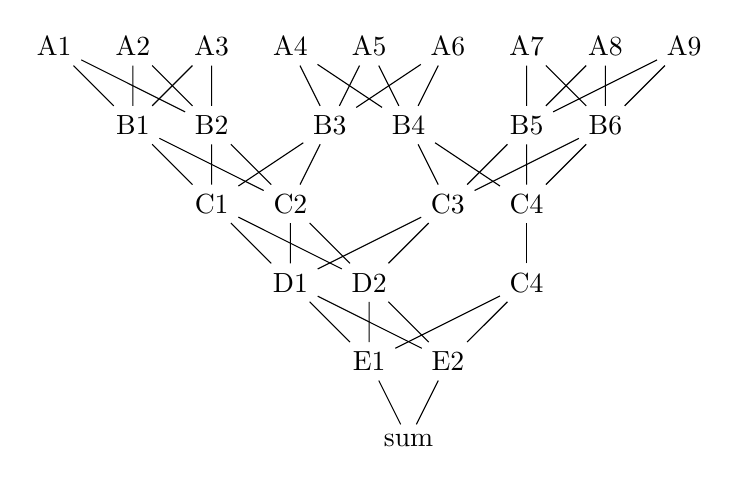
\begin{tikzpicture}
\node (A1) at (0,0) {A1};
\node (A2) at (1,0) {A2};
\node (A3) at (2,0) {A3};
\node (A4) at (3,0) {A4};
\node (A5) at (4,0) {A5};
\node (A6) at (5,0) {A6};
\node (A7) at (6,0) {A7};
\node (A8) at (7,0) {A8};
\node (A9) at (8,0) {A9};

\node (B1) at (1,-1) {B1};
\node (B2) at (2,-1) {B2};
\node (B3) at (3.5,-1) {B3};
\node (B4) at (4.5,-1) {B4};
\node (B5) at (6,-1) {B5};
\node (B6) at (7,-1) {B6};

\draw (B1) --(A1) --(B2);
\draw (B1) --(A2) --(B2);
\draw (B1) --(A3) --(B2);
\draw (B3) --(A4) --(B4);
\draw (B3) --(A5) --(B4);
\draw (B3) --(A6) --(B4);
\draw (B5) --(A7) --(B6);
\draw (B5) --(A8) --(B6);
\draw (B5) --(A9) --(B6);

\node (C1) at (2,-2) {C1};
\node (C2) at (3,-2) {C2};
\node (C3) at (5,-2) {C3};
\node (C4) at (6,-2) {C4};

\draw (C1) --(B1) --(C2);
\draw (C1) --(B2) --(C2);
\draw (C1) --(B3) --(C2);
\draw (C3) --(B4) --(C4);
\draw (C3) --(B5) --(C4);
\draw (C3) --(B6) --(C4);

\node (D1) at (3,-3) {D1};
\node (D2) at (4,-3) {D2};
\node (D3) at (6,-3) {C4};

\draw (D1) --(C1) --(D2);
\draw (D1) --(C2) --(D2);
\draw (D1) --(C3) --(D2);
\draw (D3) --(C4);

\node (E1) at (4,-4) {E1};
\node (E2) at (5,-4) {E2};

\draw (E1) --(D1) --(E2);
\draw (E1) --(D2) --(E2);
\draw (E1) --(D3) --(E2);

\node (sum) at (4.5,-5) {sum};

\draw (E1) --(sum) --(E2);
\end{tikzpicture}

On obtient ainsi une profondeur totale en \textbf{NAND} de $4 s - 2 + 12(3p - 2) = 4s + 36p -22$, or $p = \lceil \log_3(nb) \rceil$ donc on a bien une profondeur en \textbf{NAND} de $4s + 36\log_3(nb) -22$.
\end{proof}

\end{subsection}
\begin{subsection}{Prendre la valeur absolue dans $\ZZq$}
	Rappelons que la valeur absolue d'un élément $x\in \ZZq$ est par
	définition la valeur absolue de son représentant dans $\rrbracket -q/2,
	q/2\rrbracket$. 
	
	Dans notre situation, $q = 2^l$ et nous représentons $a\in \ZZq$ par une liste de
	taille $l-1$\footnote{Pour des raisons techniques, il est en fait
	représenté par une liste de taille $l$, mais nous ne faisons alors pas
	attention au dernier bit}, le bit de poids faible étant à gauche.
	Autrement dit:
\[ a = [a_0, \cdots, a_{l-1}] \quad \text{pour représenter } a = \sum_{i=0}^{l-1} a_i 2^i\]

	On peut alors calculer ainsi en binaire la valeur absolue de $a$:

\vspace{0.5cm}
\begin{lstlisting}
if $a_{l-1} = 0$: 
	# on a $a < q/2$
	return $a$
else:
	# on a $a < q/2$, alors $|a - q| = \left( (2^l - 1) - a + 1 \right)$
	$a$ = [NOT($a_i$) for $i$ in range($l$)]
	return basic_sum($a$, $1$)
\end{lstlisting}

Toutefois, il n'est pas possible de faire de conditions homomorphiquement,
ainsi, afin de pouvoir l'écrire homomorphiquement, on va en fait considérer 
le code suivant:

\vspace{0.5cm}
\begin{lstlisting}
$b$ = basic_sum([NOT($a_i$) for $i$ in range($l$)], 1)
return [($a_{l-1} \land a_i) \lor (\overline{a_{l_1}} \land b_i)$  for $i$ in range($l$)]
\end{lstlisting}

On peut alors utiliser les comptes déjà fait, notamment concernant la
	profondeur en NAND de \textbf{basic\_sum}, pour conclure:
\begin{prop}
	En conservant nos conventions pour la représentation des données, prendre la valeur absolue
	d'un élément $a\in \ZZq$ demande une profondeur de $4s + 2$ NAND.
\end{prop}
\end{subsection}
En additionnant nos différents comptes, on peut alors conclure:

\begin{prop}
	On peut effectuer l'algorithme \textbf{Dec} avec une profondeur de
	RESULTAT NAND.
\end{prop}
	




\end{section}
